%!TEX TS-program = lualatex
%!TEX encoding = UTF-8 Unicode

\documentclass{article}
\usepackage[left=0.5in,right=0.5in,top=1in]{geometry}     

\usepackage[parfill]{parskip}

\usepackage{pdflscape}

\usepackage{fontspec}
\def\mainfont{Linux Libertine O}
\setmainfont[Ligatures={TeX, Common}, BoldFont={* Bold}, ItalicFont={* Italic}, Fractions ={On}, Numbers={OldStyle,Proportional}]{\mainfont}
%\setmonofont[Scale=MatchLowercase]{Inconsolata} 
%\setsansfont[Scale=MatchLowercase]{Linux Biolinum O} 
\usepackage{microtype}

\usepackage{graphicx}
	\graphicspath{%
	{/Users/goby/Pictures/teach/348/exams/}}%

\begin{document}
\thispagestyle{empty}

{\fontsize{20pt}{24pt}\selectfont

Figure for page 3, questions 6–11 and extra credit about ocean zones.

\begin{center}
	\includegraphics[width=\textwidth]{exam1_figure}
\end{center}

\newpage
\thispagestyle{empty}

Figure for page 4, question 12 about crabs in Africa. 

\begin{center}
	\includegraphics[height=0.9\textheight]{africa_schulte}
\end{center}
}
\newpage
\thispagestyle{empty}

\begin{landscape}
%\newgeometry{right=0.5in}

{\fontsize{20pt}{24pt}\selectfont
Figure for pages 5–6, question 13a and b about snaggletooth.
}

\begin{center}
	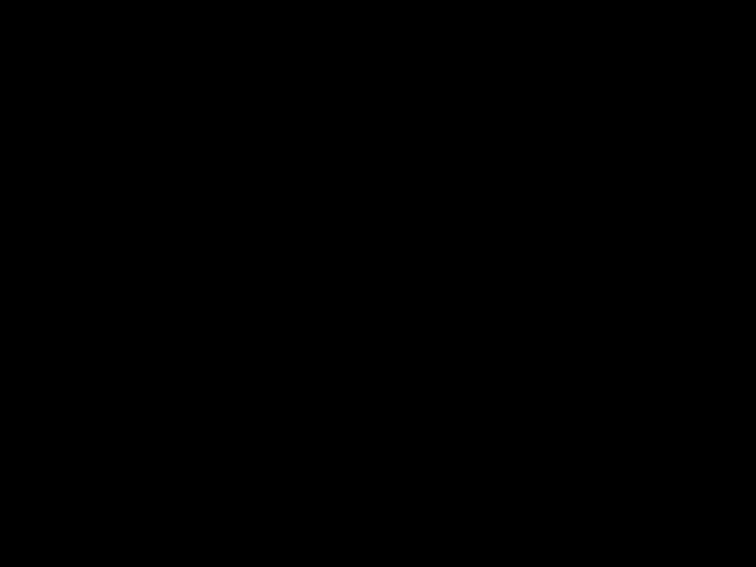
\includegraphics[height=0.92\textheight]{exam1_astronesthes}
\end{center}


\end{landscape}

\end{document}